\documentclass[tikz,border=2pt]{standalone}
\usepackage{amsmath}
\usepackage{pgfplots}
\pgfplotsset{compat=1.18}
\usetikzlibrary{arrows.meta,decorations.pathreplacing}
\begin{document}
% Weak duality on Example 5.1: primal feasible values c^T x at x=(0,0),(4,0),(4,3) are 0, 12, 27;
% dual feasible values b^T y at y=(0,2,1),(0,0,3) are 42, 54; every primal value lies below every dual value,
% so 27 <= Z* <= W* <= 42 (gap 42-27=15).
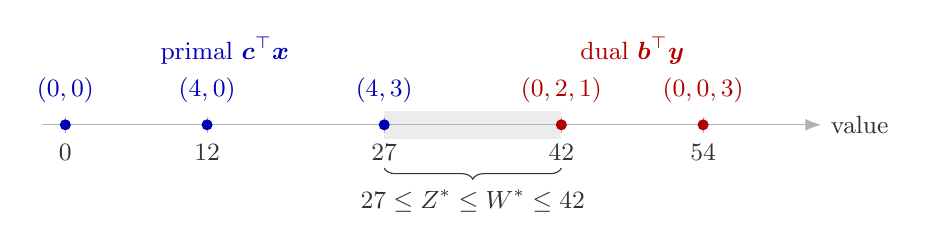
\begin{tikzpicture}[font=\small, >={Latex[length=2mm]}, x=0.15cm, y=1cm]
  % bracket band for the optima
  \fill[gray!15] (27,-0.18) rectangle (42,0.18);
  % axis
  \draw[gray!60, ->] (-2,0) -- (64,0) node[anchor=west, gray!40!black] {value};
  \foreach \v in {0,12,27,42,54} {
    \draw[gray!60] (\v,0.1) -- (\v,-0.1);
    \node[gray!40!black, anchor=north] at (\v,-0.12) {$\v$};
  }
  % primal feasible values
  \foreach \v/\lab in {0/{(0,0)}, 12/{(4,0)}, 27/{(4,3)}} {
    \fill[blue!70!black] (\v,0) circle (2pt);
    \node[blue!70!black, anchor=south] at (\v,0.15) {$\lab$};
  }
  \node[blue!70!black, anchor=south] at (13.5,0.65) {primal $\boldsymbol{c}^{\top}\boldsymbol{x}$};
  % dual feasible values
  \foreach \v/\lab in {42/{(0,2,1)}, 54/{(0,0,3)}} {
    \fill[red!70!black] (\v,0) circle (2pt);
    \node[red!70!black, anchor=south] at (\v,0.15) {$\lab$};
  }
  \node[red!70!black, anchor=south] at (48,0.65) {dual $\boldsymbol{b}^{\top}\boldsymbol{y}$};
  % where the optima must lie
  \draw[gray!40!black, decorate, decoration={brace, mirror, amplitude=4pt}] (27,-0.55) -- (42,-0.55);
  \node[gray!40!black, anchor=north] at (34.5,-0.7) {$27\leq Z^{\ast}\leq W^{\ast}\leq42$};
\end{tikzpicture}
\end{document}
